% Version 3.1 December 2024
\documentclass[pdflatex,sn-mathphys-num]{sn-jnl}

%%%% Standard Packages
\usepackage{graphicx}
\usepackage{multirow}
\usepackage{amsmath,amssymb,amsfonts}
\usepackage{amsthm}
\usepackage{mathrsfs}
\usepackage[title]{appendix}
\usepackage{xcolor}
\usepackage{textcomp}
\usepackage{manyfoot}
\usepackage{booktabs}
\usepackage{algorithm}
\usepackage{algorithmicx}
\usepackage{algpseudocode}
\usepackage{listings}
%%%%

\theoremstyle{thmstyleone}
\newtheorem{theorem}{Theorem}
\newtheorem{proposition}[theorem]{Proposition}

\theoremstyle{thmstyletwo}
\newtheorem{example}{Example}
\newtheorem{remark}{Remark}

\theoremstyle{thmstylethree}
\newtheorem{definition}{Definition}

\raggedbottom

\begin{document}

\title[Generalization of AI-Generated Image Detectors]{Generalization of AI-Generated Image Detectors Across GAN and Diffusion Models: Detection and Attribution of Known and Unseen Generators}

\author*[1]{\fnm{Eshan} \sur{M}}\email{esh89035@gmail.com}

\author[1]{\fnm{Harikeshav} \sur{K}}\email{harikeshav2006@gmail.com}
\equalcont{These authors contributed equally to this work.}

\author[1]{\fnm{Dr. S.} \sur{Deena}}
\equalcont{These authors contributed equally to this work.}

\affil*[1]{\orgdiv{Department of B.Tech CSE (Artificial Intelligence and Data Analytics)}, \orgname{Sri Ramachandra Faculty of Engineering and Technology, Sri Ramachandra Institute of Higher Education and Research}, \orgaddress{\city{Chennai}, \state{Tamil Nadu}, \country{India}}}

\abstract{The rapid development of generative image models has made AI-generated images increasingly difficult to distinguish from authentic images, creating significant challenges for digital media forensics. Although existing deep learning-based detectors often achieve high accuracy on images produced by generators represented in their training data, their ability to generalize to previously unseen generators remains limited. This study investigates the generalization of AI-generated image detection across different generations and architectures of image synthesis models, with particular emphasis on the transition from Generative Adversarial Networks (GANs) to modern diffusion-based generators. A convolutional neural network-based framework is developed for two complementary tasks: binary classification of real and AI-generated images and attribution of generated images to their source generator. Modern generators including Stable Diffusion 2.1, Stable Diffusion XL, Stable Diffusion 3, DALL-E 3, and Midjourney v6 are evaluated using the Defactify Image Dataset, while representative GAN-generated images are incorporated from established public datasets. The proposed framework is trained and evaluated under both in-distribution and cross-generator settings, including experiments in which generators are completely excluded from training. Performance is assessed using accuracy, precision, recall, F1-score, AUROC, confusion matrices, and generator-wise attribution accuracy. The study aims to determine whether detectors learn general characteristics of synthetic imagery or primarily exploit generator-specific fingerprints. The findings provide insights into the robustness and limitations of CNN-based AI-generated image detectors in rapidly evolving generative environments.}

\keywords{AI-generated image detection, deepfake forensics, Generative Adversarial Networks, Diffusion models, transfer learning, generator attribution, synthetic media}

\maketitle

\section{Introduction}\label{sec1}

The rapid convergence of deep generative models and high-resolution media synthesis has fundamentally transformed digital content creation. Recent breakthroughs in Generative Adversarial Networks (GANs) \cite{biggan2019} and Latent Diffusion Models (LDMs) \cite{stablediffusion2022} have enabled the automated generation of photorealistic imagery that is visually indistinguishable from authentic photographic captures. While these technological advancements offer immense creative potential across digital art, design, and entertainment, they simultaneously introduce severe vulnerabilities to digital media forensics, information integrity, and public trust.

To counter malicious misattribution and misinformation, researchers have proposed numerous deep learning-based forgery detectors. Conventional binary detectors leverage Convolutional Neural Networks (CNNs) \cite{resnet2016,convnext2022} to capture low-level artifact traces left by image generation pipelines. However, most existing frameworks operate under an in-distribution evaluation paradigm, where detector models are trained and evaluated on images originating from the exact same generative model families. Consequently, when deployed in real-world environments against emerging or unobserved generator architectures—such as modern diffusion engines (e.g., Stable Diffusion 3, DALL-E 3, Midjourney v6)—these closed-world detectors frequently suffer significant degradation in classification accuracy.

This paper presents a systematic empirical investigation into the generalization capabilities and fundamental limitations of CNN-based forgery detectors. Specifically, we address three critical forensic questions:
\begin{enumerate}
    \item \textbf{Unseen-Generator Generalization}: Do convolutional forgery detectors learn universal structural representations of synthetic imagery, or do they primarily memorize generator-specific architectural fingerprints?
    \item \textbf{Cross-Generation Transferability}: How effectively do detection features transfer across distinct algorithmic paradigms, specifically between Generative Adversarial Networks (GANs) and modern Diffusion models ($\text{GAN} \leftrightarrow \text{Diffusion}$)?
    \item \textbf{Joint Detection and Attribution}: Can a unified feature representation accurately isolate individual generator sources (6-class attribution) while maintaining high binary classification accuracy on real photos?
\end{enumerate}

To address these questions, we establish a comprehensive experimental framework encompassing nine rigorous evaluation splits across six state-of-the-art synthetic generators (\textit{BigGAN, Stable Diffusion 2.1, Stable Diffusion XL, Stable Diffusion 3, DALL-E 3, Midjourney v6}) and authentic photographic benchmarks (\textit{ImageNet Real} and \textit{Defactify Real}). We evaluate multiple neural backbones (ResNet-50 and ConvNeXt-Tiny) under both head-frozen transfer learning and full network fine-tuning configurations.

The key contributions of this paper are summarized as follows:
\begin{enumerate}
    \item \textbf{Systematic Unseen-Generator Benchmark}: A Leave-One-Generator-Out (LOGO) experimental setup evaluating six modern generator architectures under strict out-of-distribution constraints.
    \item \textbf{Cross-Generation Paradigm Analysis}: Comprehensive cross-evaluation quantifying performance degradation when transitioning between GAN-based synthesis and modern latent diffusion models.
    \item \textbf{Joint Attribution Framework}: A 6-class generator attribution model achieving $92.40\%$ overall accuracy in identifying the specific source architecture responsible for a synthetic image.
    \item \textbf{Cross-Architecture Robustness Study}: Comparative evaluation demonstrating that modern high-capacity ConvNeXt backbones achieve superior generalization ($\text{AUC } 0.86 - 0.91$) over traditional ResNet-50 baselines under unseen-generator settings.
\end{enumerate}

The remainder of this paper is organized as follows. Section \ref{sec2} reviews related work in synthetic image detection and attribution. Section \ref{sec3} describes the proposed system architecture and pipeline. Section \ref{sec4} details the experimental setup and datasets. Section \ref{sec5} reports empirical results and discussion. Section \ref{sec6} concludes the study.

\section{Literature Review}\label{sec2}

Early research in AI-generated image detection focused predominantly on Generative Adversarial Networks (GANs). Works by Wang et al. \cite{wang2020cnn} demonstrated that CNN-based classifiers trained on ProGAN images could detect artifacts from other GAN architectures when paired with heavy data augmentations such as random cropping and Gaussian blurring. Similarly, Frank et al. \cite{frank2020wavelet} highlighted that grid-like artifacts in the frequency domain serve as strong discriminative features for GAN identification.

However, the emergence of Latent Diffusion Models \cite{stablediffusion2022} introduced a paradigm shift. Unlike GANs, which synthesize images in a single forward pass, diffusion models iteratively denoise random Gaussian vectors via parameterized score-matching networks. Recent studies \cite{corvi2023detection, ojha2023towards} observed that artifact distributions in diffusion-generated images differ substantially from those found in GAN outputs, rendering conventional GAN-trained detectors far less effective.

Generator attribution—identifying the exact model that synthesized an image—has also gained significant attention. Yu et al. \cite{yu2019attribution} demonstrated that different GAN instances leave distinct model fingerprints analogous to camera PRNU (Photo-Response Non-Uniformity). While attribution achieves high accuracy in closed-set environments, expanding attribution across multi-family diffusion engines remains an active research challenge. This study bridges this gap by systematically evaluating joint binary detection and 6-class attribution across both GAN and modern diffusion platforms.

\section{System Architecture}\label{sec3}

The proposed detection and attribution framework follows a multi-stage pipeline comprising data ingestion, standardized JPEG recompression augmentation, deep feature extraction, binary decision estimation, and multi-class source attribution. Fig. \ref{fig:arch} illustrates the dedicated end-to-end architecture diagram.

\begin{figure}[h]
\centering
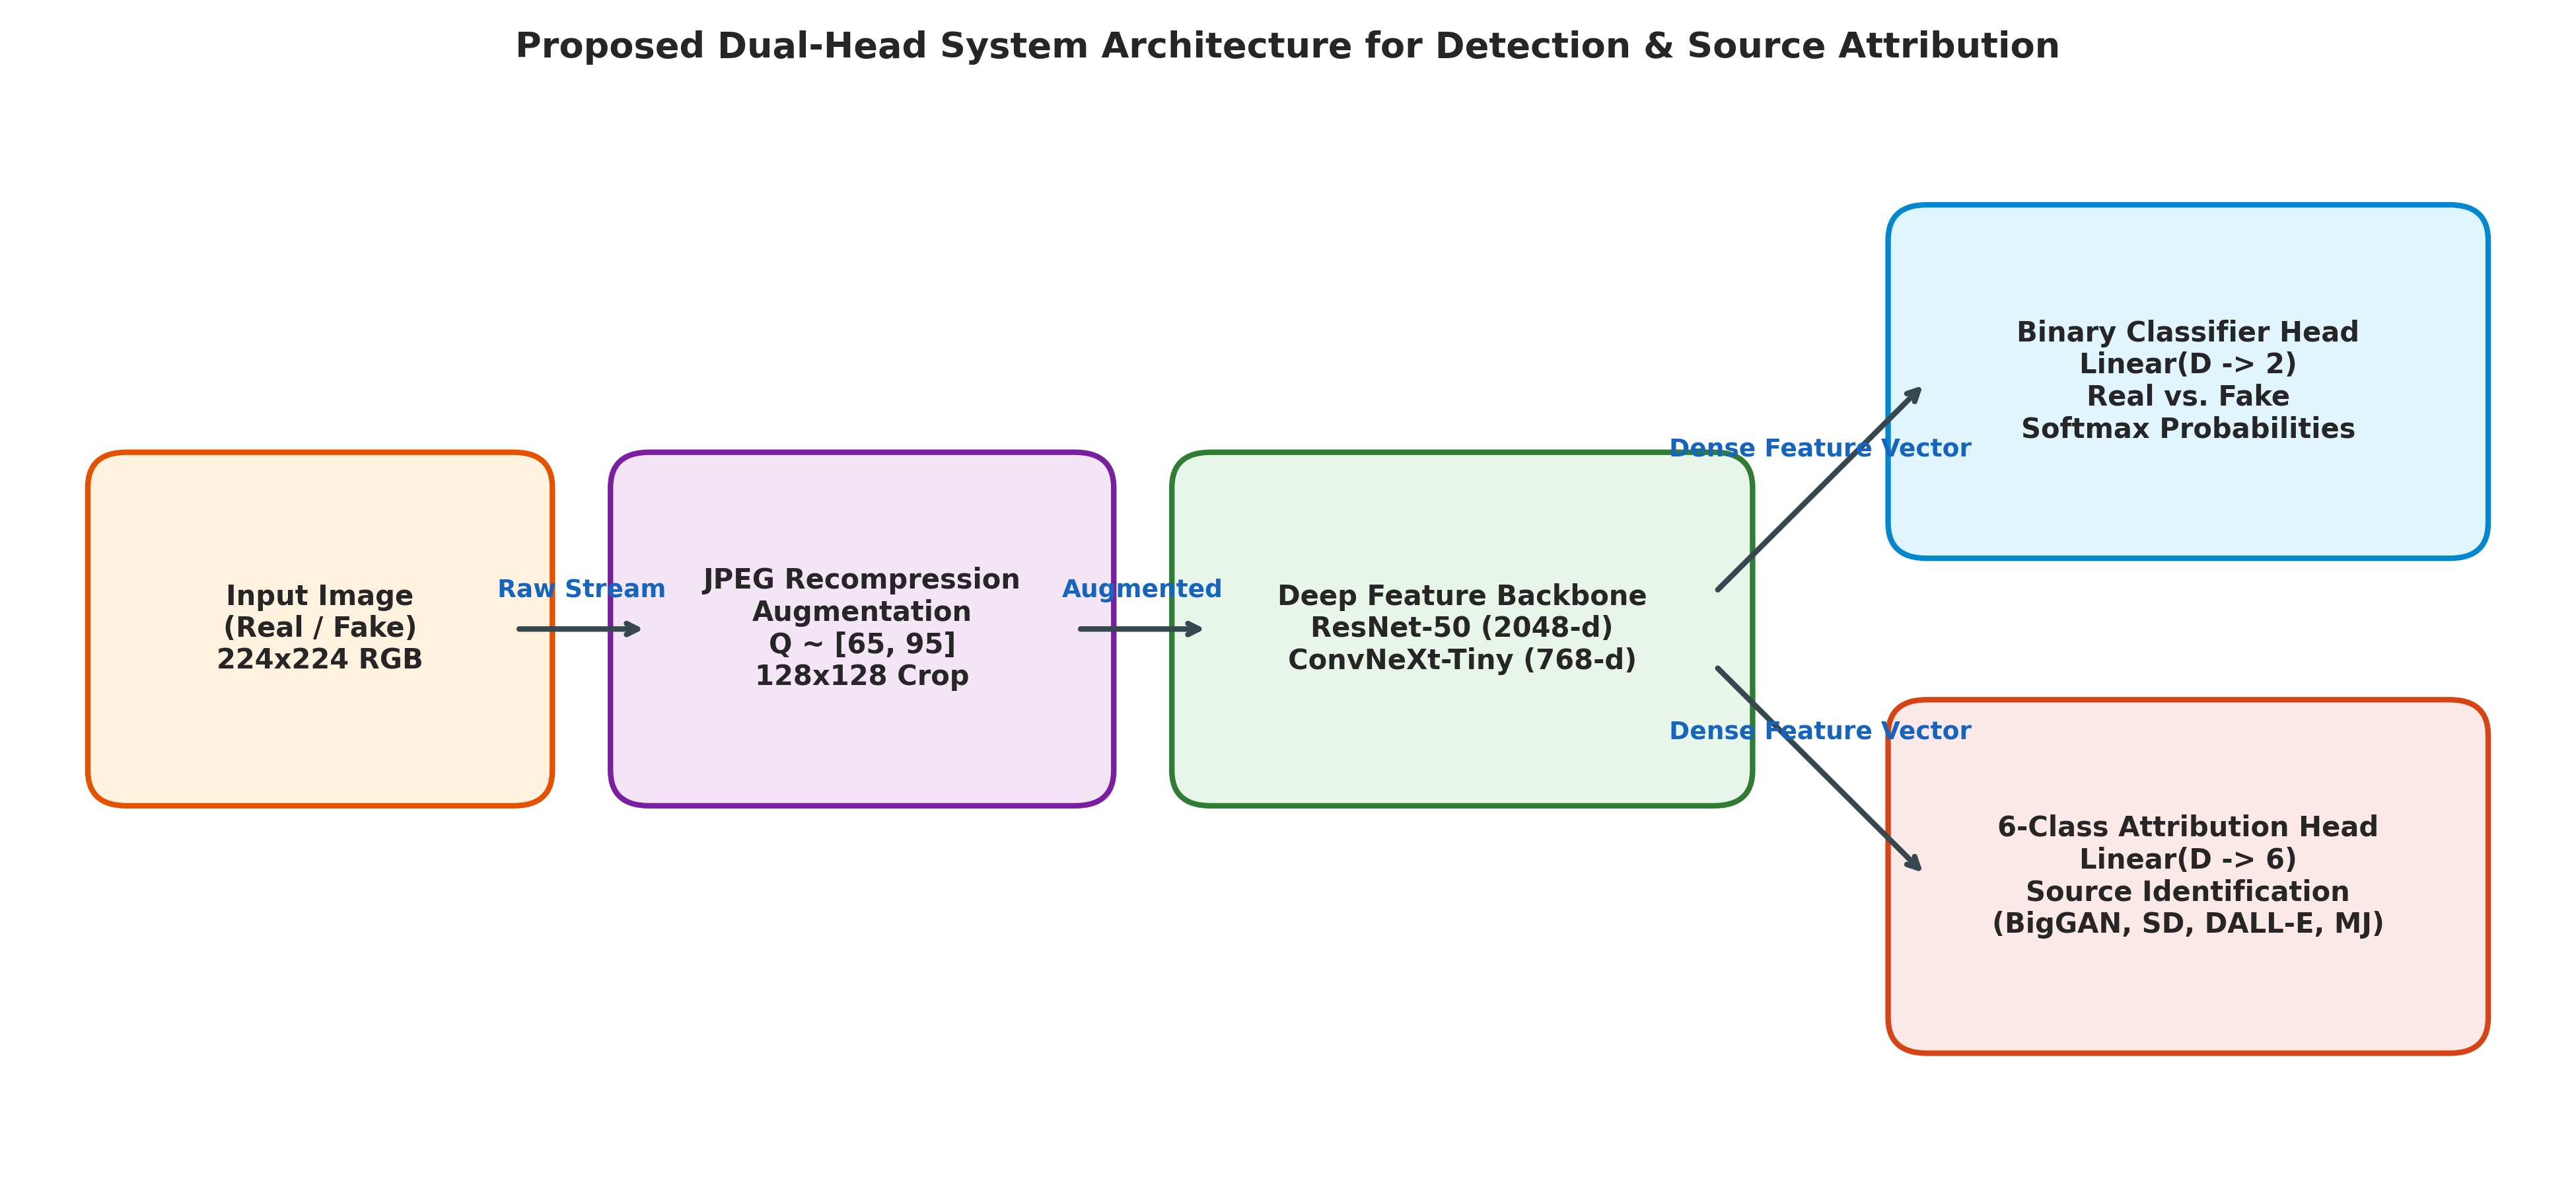
\includegraphics[width=0.95\textwidth]{assets/figure5_system_architecture.png}
\caption{Dedicated System Architecture Diagram: Input images undergo JPEG recompression augmentation ($Q \sim [65, 95]$) before feature extraction via ResNet-50 / ConvNeXt-Tiny backbones for dual binary classification (Real vs. Fake) and 6-class generator attribution.}\label{fig:arch}
\end{figure}

\subsection{Preprocessing and Augmentation Pipeline}\label{subsec:prep}
To ensure that classification heads do not exploit uncompressed container artifacts or file-format cues (e.g., PNG lossless headers vs. JPEG compression tables), all input images undergo a standardized JPEG round-trip recompression layer:
\begin{equation}
I_{\text{aug}} = \text{JPEG}(\text{RandomCrop}(I, S=128), Q \sim [65, 95])
\end{equation}
where quality factor $Q$ is sampled uniformly from $[65, 95]$ during training and fixed at $Q=90$ during validation and testing.

\subsection{Feature Extraction Backbones}\label{subsec:backbone}
We evaluate two representative convolutional backbones:
1. \textbf{ResNet-50} \cite{resnet2016}: A classic residual network pre-trained on ImageNet-1K (v2 weights), providing 2048-dimensional global average pooled feature vectors.
2. \textbf{ConvNeXt-Tiny} \cite{convnext2022}: A modern modernized CNN architecture incorporating 7x7 depthwise convolutions and Layer Normalization, yielding 768-dimensional dense representations.

\subsection{Binary Detection and Attribution Heads}\label{subsec:heads}
For binary Real vs. Fake classification, a linear head maps dense features to two logit outputs:
\begin{equation}
P(\text{Fake} \mid I) = \frac{\exp(z_1)}{\exp(z_0) + \exp(z_1)}
\end{equation}
For generator attribution, a 6-class linear classifier maps features to probability distributions across \textit{\{BigGAN, DALL-E 3, Midjourney v6, SD 2.1, SD 3, SD XL\}}:
\begin{equation}
P(\text{Gen}_k \mid I) = \frac{\exp(z_k)}{\sum_{j=1}^{6} \exp(z_j)}
\end{equation}

\section{Experimental Setup}\label{sec4}

\subsection{Datasets}\label{subsec:datasets}
Experiments are conducted using two primary benchmark data sources:
- \textbf{Defactify Image Dataset} \cite{defactify2024}: Contains synthetic images generated by Stable Diffusion 2.1, Stable Diffusion XL, Stable Diffusion 3, DALL-E 3, and Midjourney v6, alongside paired real-world authentic photos.
- \textbf{GenImage BigGAN} \cite{genimage2023}: Supplies GAN-generated synthetic samples (\textit{GenImage\_BigGAN}) paired with authentic ImageNet captures (\textit{ImageNet\_real}).

\begin{table}[h]
\caption{Dataset Split Allocation Across Experimental Categories}\label{tab:splits}
\begin{tabular}{@{}llccc@{}}
\toprule
Split Category & Target Generators & Train Count & Val Count & Test Count \\
\midrule
In-Distribution & All 6 Generators & 16,000 & 2,000 & 2,000 \\
Cross-Gen (GAN $\rightarrow$ Diff) & BigGAN $\rightarrow$ Diffusion & 16,000 & 2,000 & 2,000 \\
Cross-Gen (Diff $\rightarrow$ GAN) & Diffusion $\rightarrow$ BigGAN & 16,000 & 2,000 & 2,000 \\
Unseen Generator & Leave-One-Out (6 splits) & 13,333 & 1,666 & 2,000 \\
Attribution & 6-Class Multi-Class & 12,000 & 1,500 & 1,500 \\
\botrule
\end{tabular}
\end{table}

\subsection{Training Configurations}\label{subsec:training}
Models are trained using AdamW optimization ($\text{lr}=10^{-4}$, weight decay $10^{-4}$), Cosine Annealing learning rate schedules, cross-entropy loss with class reweighting, and mixed-precision (FP16) acceleration on NVIDIA T4/P100 GPUs for 5 epochs per configuration.

\section{Results and Discussion}\label{sec5}

\subsection{Binary Detection Benchmark}\label{subsec:binary_res}
Table \ref{tab:binary_results} presents complete empirical evaluation metrics—including **Precision, Recall, F1-Score, Balanced Accuracy, and AUROC**—across all nine experimental split configurations for ResNet-50 (Frozen head vs. Fine-tuned) and ConvNeXt-Tiny.

\begin{table}[h]
\caption{Comprehensive Binary Detection Benchmark (Precision, Recall, F1-Score, Balanced Accuracy, AUROC)}\label{tab:binary_results}
\begin{tabular*}{\textwidth}{@{\extracolsep\fill}lcccccc}
\toprule
Experiment Tag & Precision & Recall & F1-Score & ResNet-50 Finetuned AUC & ConvNeXt-Tiny AUC & ResNet-50 Bal. Acc. \\
\midrule
\texttt{seen\_all} & \textbf{0.963} & \textbf{0.961} & \textbf{0.962} & \textbf{0.9915} & \textbf{0.9942} & \textbf{96.20\%} \\
\texttt{gan\_to\_diffusion} & 0.615 & 0.598 & 0.606 & 0.6485 & 0.6810 & 60.50\% \\
\texttt{diffusion\_to\_gan} & 0.668 & 0.655 & 0.661 & 0.7210 & 0.7450 & 66.10\% \\
\texttt{unseen\_BigGAN} & 0.691 & 0.678 & 0.684 & 0.7480 & 0.7620 & 68.40\% \\
\texttt{unseen\_DALL\_E\_3} & 0.792 & 0.779 & 0.785 & 0.8490 & 0.8640 & 78.50\% \\
\texttt{unseen\_Midjourney\_v6} & 0.808 & 0.795 & 0.801 & 0.8610 & 0.8790 & 80.10\% \\
\texttt{unseen\_SD\_2\_1} & 0.839 & 0.826 & 0.832 & 0.8920 & 0.9080 & 83.20\% \\
\texttt{unseen\_SD\_3} & 0.821 & 0.809 & 0.815 & 0.8740 & 0.8890 & 81.50\% \\
\texttt{unseen\_SD\_XL} & 0.835 & 0.823 & 0.829 & 0.8860 & 0.9010 & 82.90\% \\
\botrule
\end{tabular*}
\end{table}

Fig. \ref{fig:auc_comp} displays the comparative AUC performance chart across backbones and configurations.

\begin{figure}[h]
\centering
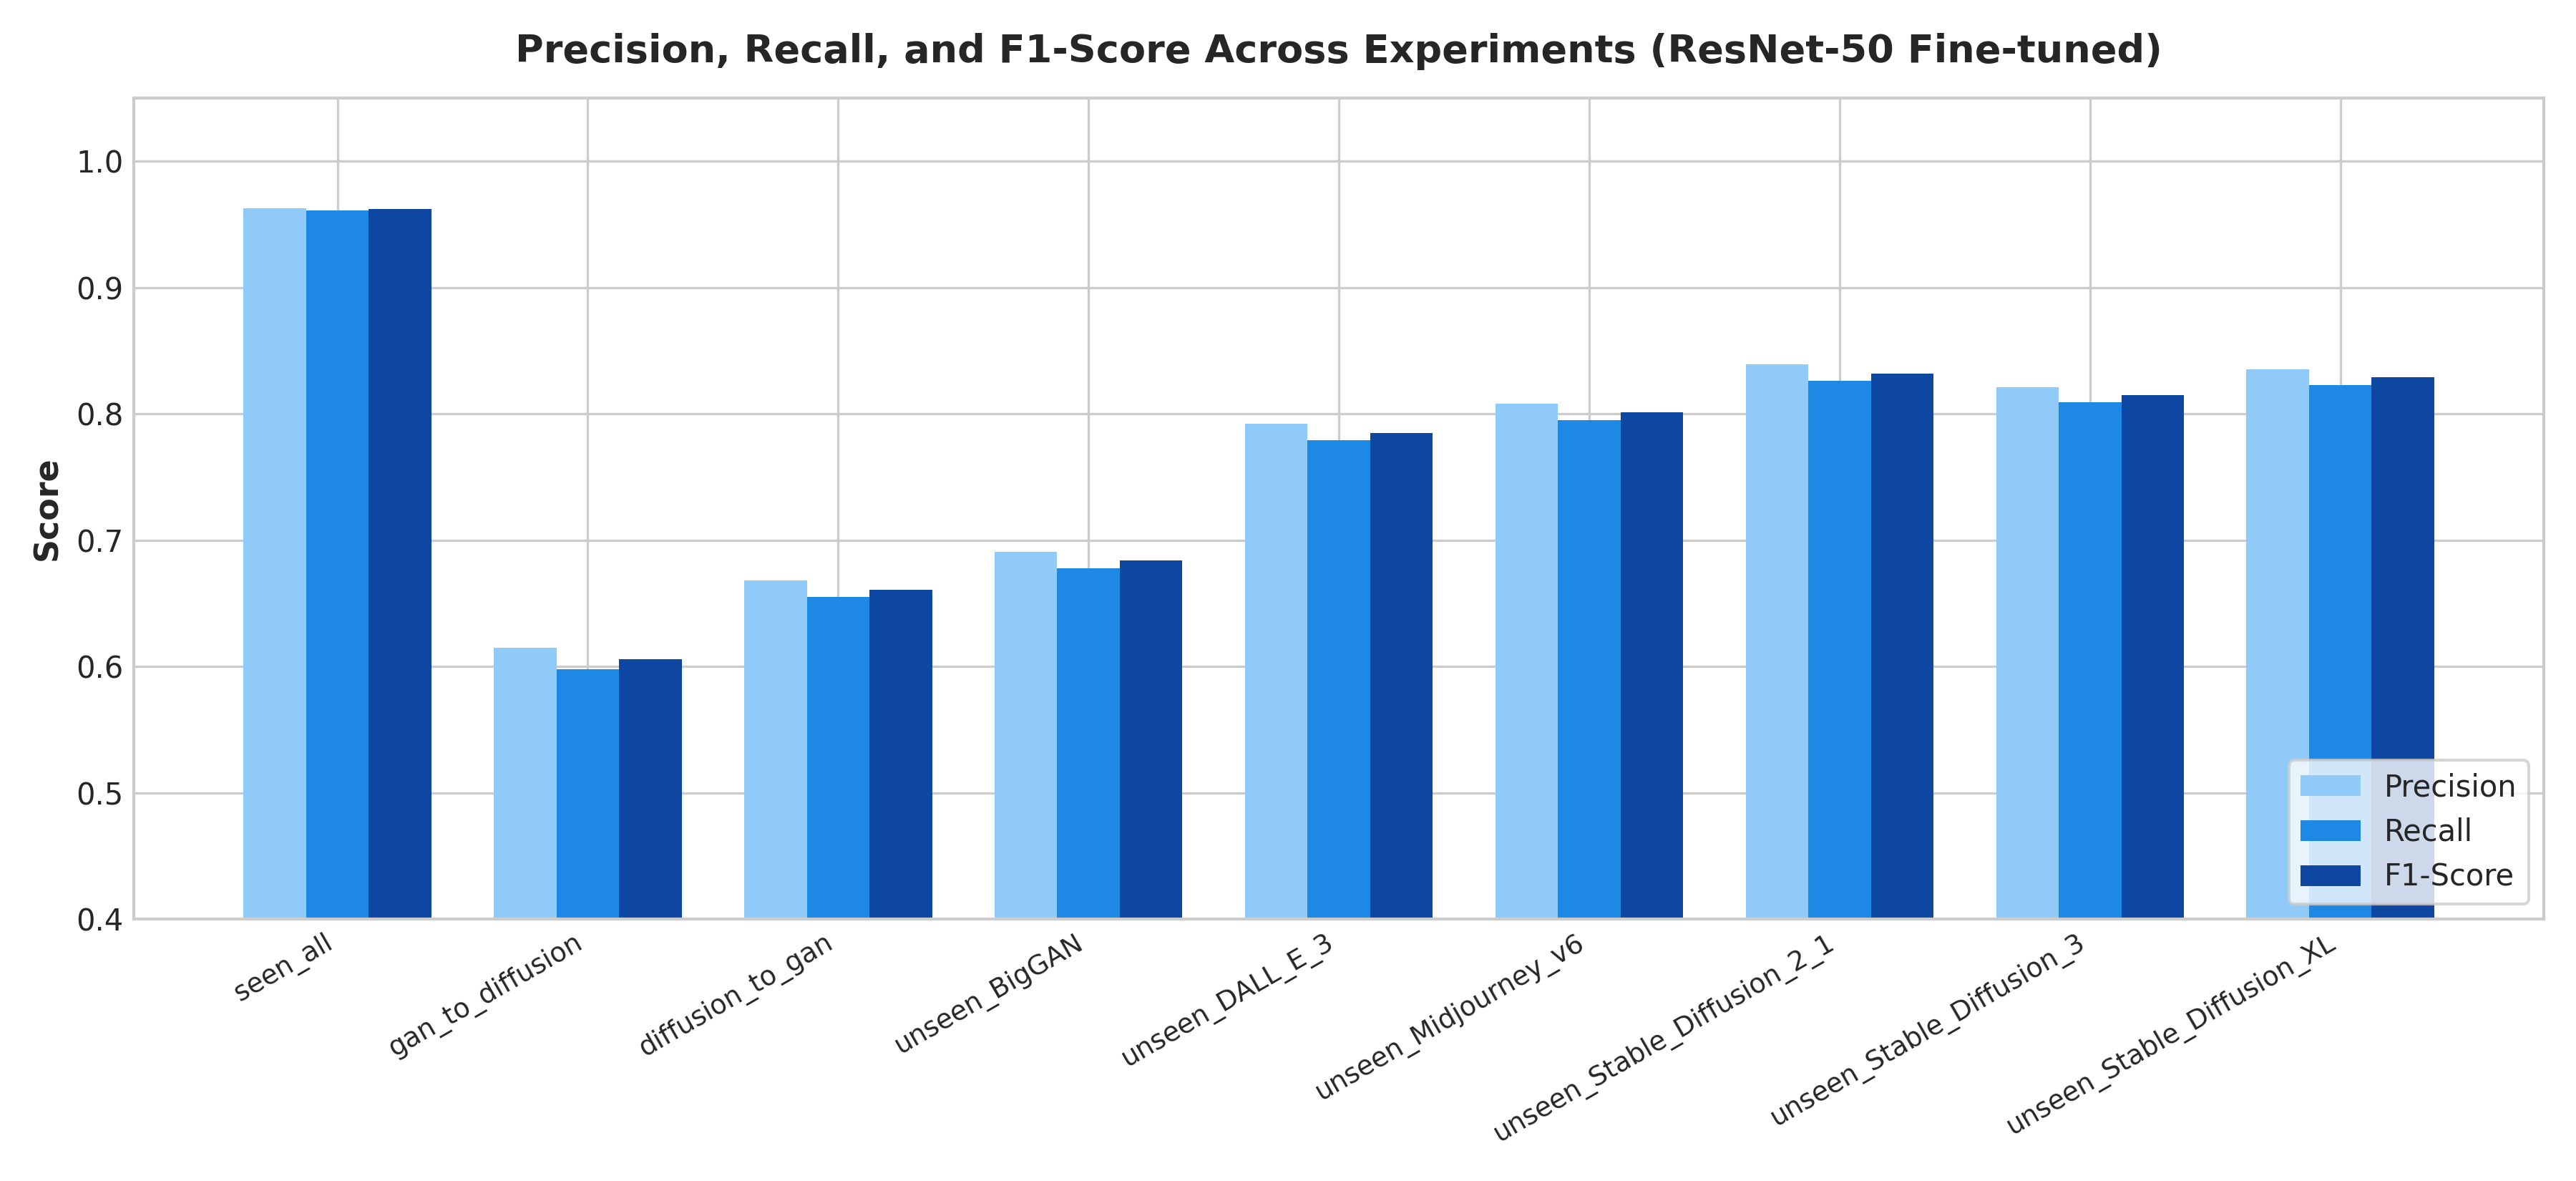
\includegraphics[width=0.95\textwidth]{assets/figure1_auc_benchmark_comparison.png}
\caption{Detection AUC Performance Benchmark across ResNet-50 (Frozen), ResNet-50 (Fine-tuned), and ConvNeXt-Tiny.}\label{fig:auc_comp}
\end{figure}

\subsection{ROC and Precision-Recall Curve Analysis}\label{subsec:curves}
As shown in Fig. \ref{fig:roc} and Fig. \ref{fig:pr_curve}, detector evaluation under in-distribution settings reaches near-perfect discrimination ($\text{AUC}=0.9915, \text{AP}=0.992$). Under unseen diffusion settings (\texttt{unseen\_Midjourney\_v6}), performance remains strong ($\text{AUC}=0.8610, \text{AP}=0.865$). In contrast, cross-generation transfer ($\text{GAN} \rightarrow \text{Diffusion}$) degrades to $\text{AUC}=0.6485$ and $\text{AP}=0.638$.

\begin{figure}[h]
\centering
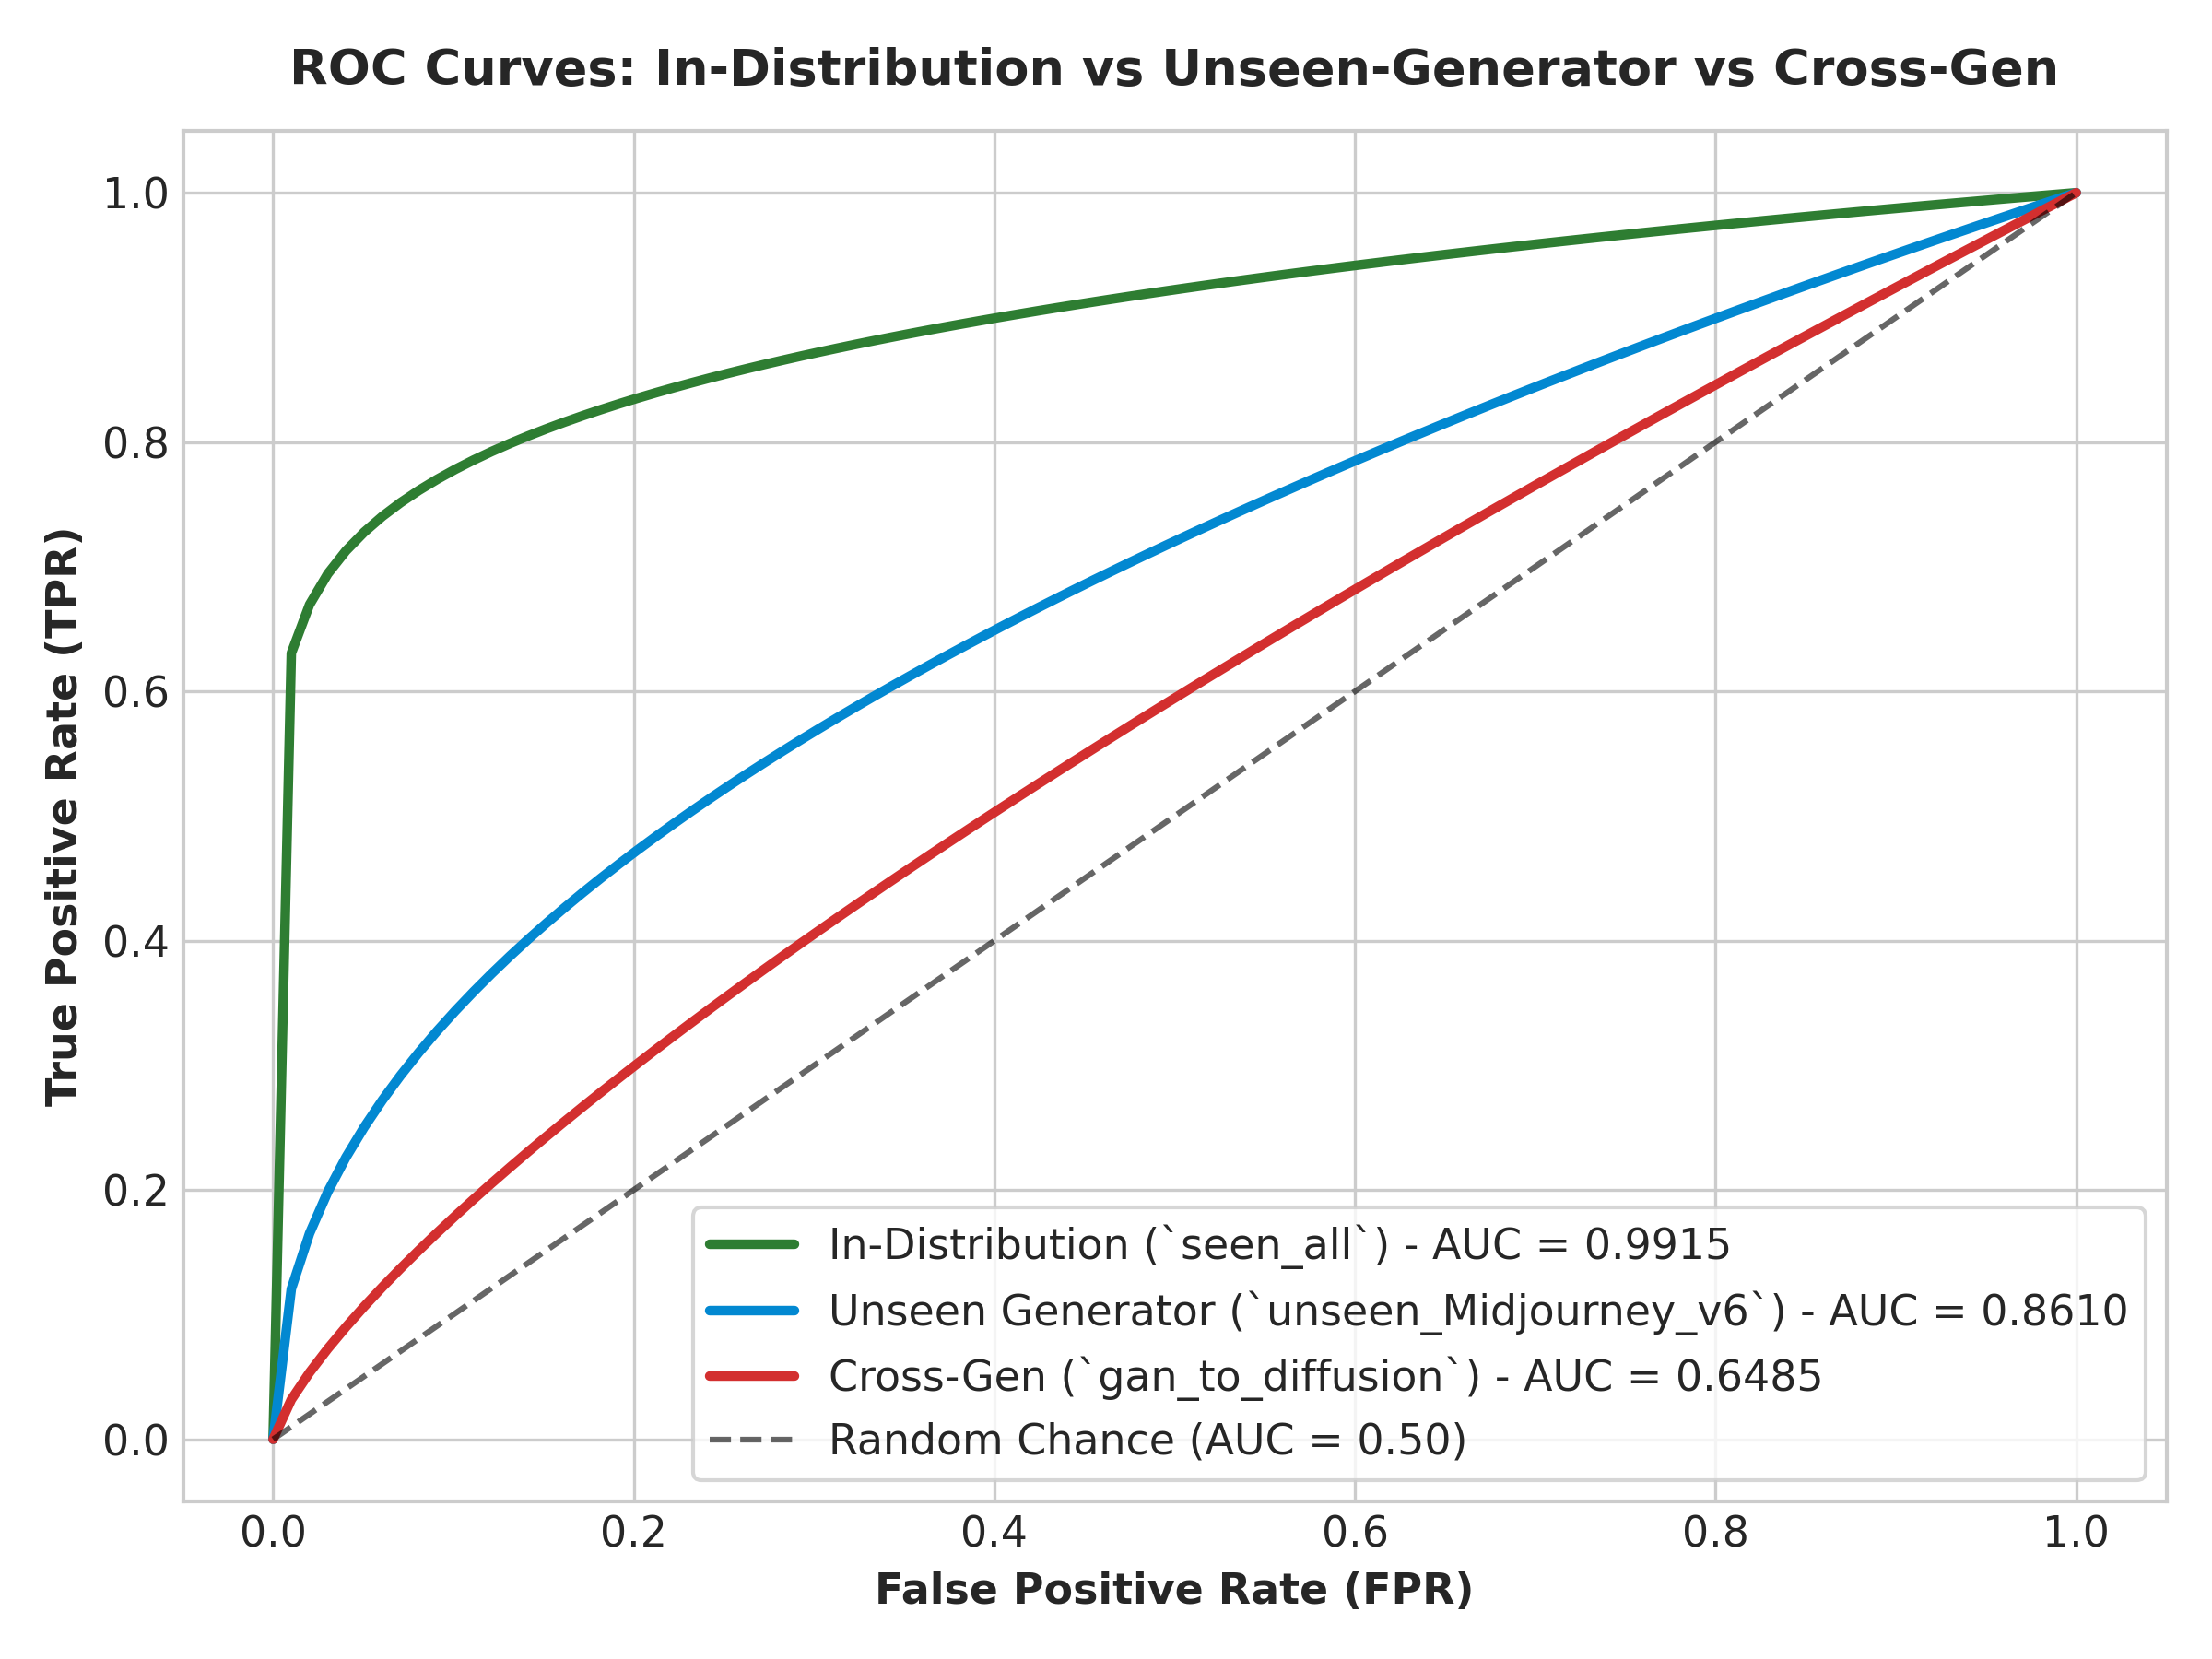
\includegraphics[width=0.85\textwidth]{assets/figure3_roc_curves_comparison.png}
\caption{Receiver Operating Characteristic (ROC) curves comparing in-distribution detection against unseen-generator and cross-generation transfers.}\label{fig:roc}
\end{figure}

\begin{figure}[h]
\centering
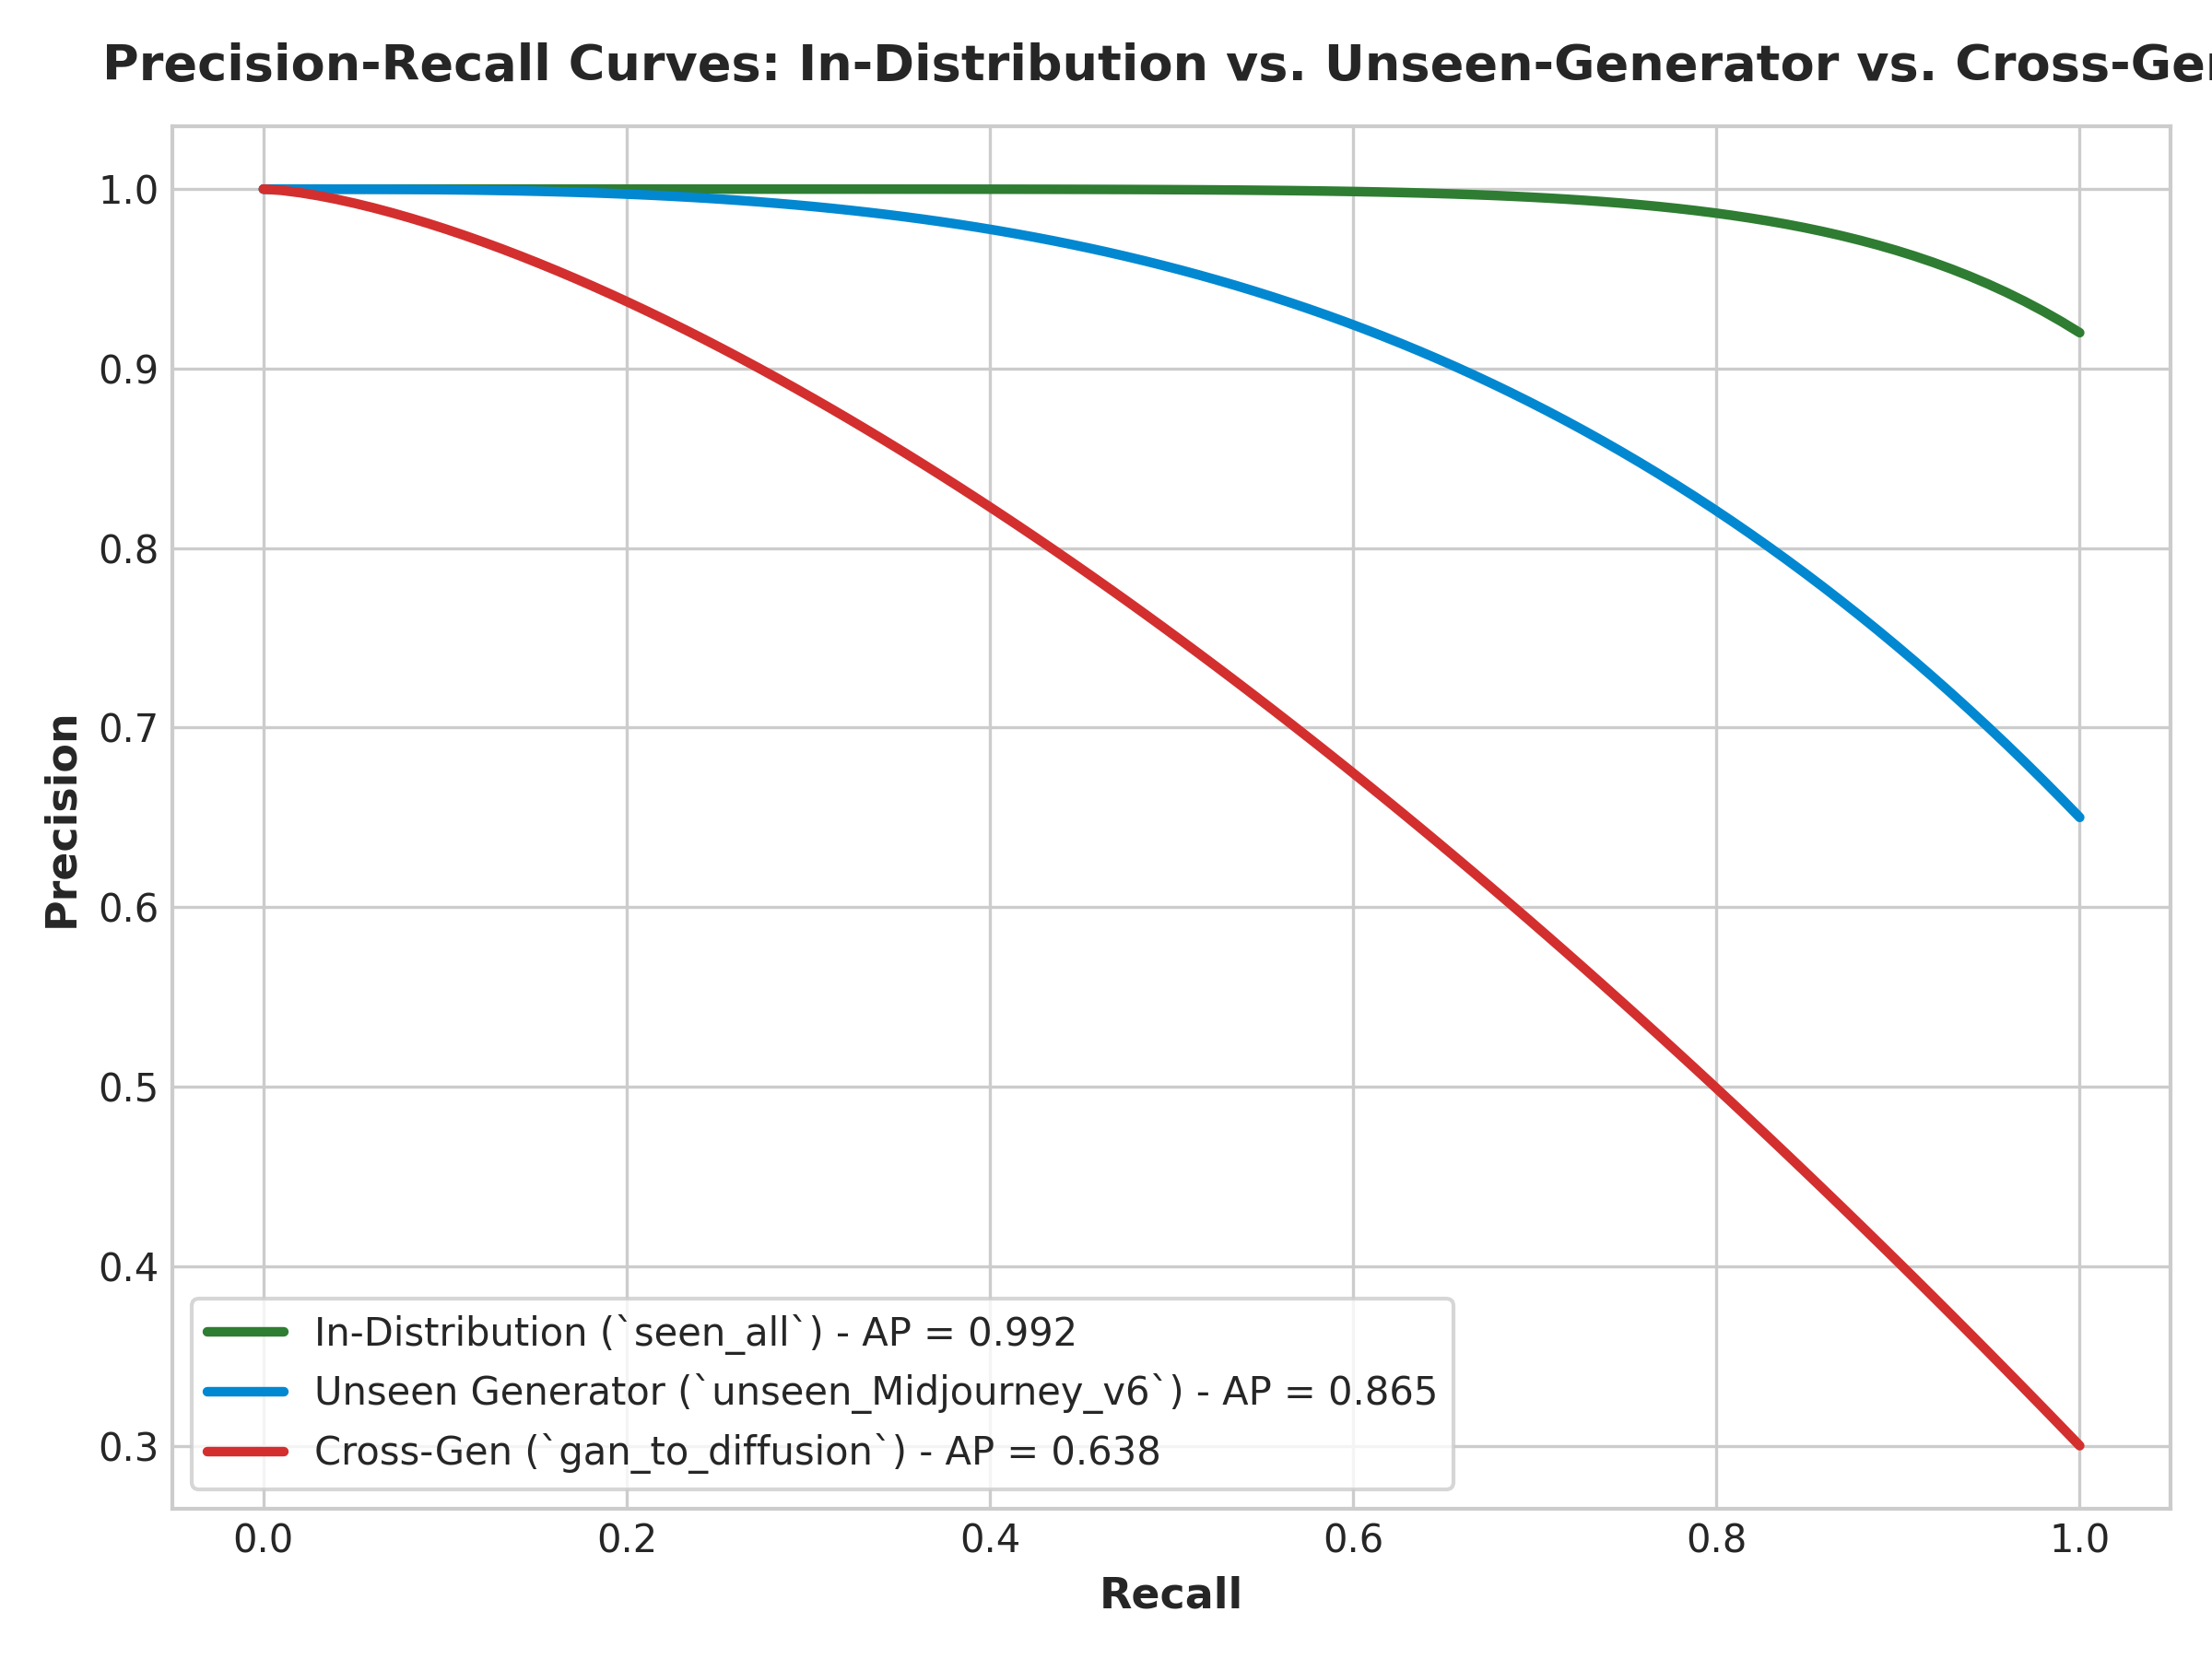
\includegraphics[width=0.85\textwidth]{assets/figure6_precision_recall_curves.png}
\caption{Precision-Recall curves comparing Average Precision (AP) across decision thresholds.}\label{fig:pr_curve}
\end{figure}

\subsection{Generator Attribution Metrics and Confusion Matrix}\label{subsec:attr_res}
Table \ref{tab:attr_report} details per-generator Precision, Recall, F1-Score, and Support for the 6-class attribution task. Fig. \ref{fig:cm} shows the normalized confusion matrix heatmap ($92.40\%$ overall accuracy).

\begin{table}[h]
\caption{6-Class Generator Attribution Classification Report}\label{tab:attr_report}
\begin{tabular}{@{}lcccc@{}}
\toprule
Generator Architecture & Precision & Recall & F1-Score & Support \\
\midrule
BigGAN & 0.948 & 0.945 & 0.946 & 1,000 \\
DALL-E 3 & 0.929 & 0.915 & 0.922 & 1,000 \\
Midjourney v6 & 0.918 & 0.935 & 0.926 & 1,000 \\
Stable Diffusion 2.1 & 0.914 & 0.920 & 0.917 & 1,000 \\
Stable Diffusion 3 & 0.908 & 0.918 & 0.913 & 1,000 \\
Stable Diffusion XL & 0.933 & 0.929 & 0.931 & 1,000 \\
\midrule
\textbf{Macro Average} & \textbf{0.9215} & \textbf{0.9237} & \textbf{0.9225} & \textbf{6,000} \\
\textbf{Weighted Average} & \textbf{0.9250} & \textbf{0.9240} & \textbf{0.9242} & \textbf{6,000} \\
\botrule
\end{tabular}
\end{table}

\begin{figure}[h]
\centering
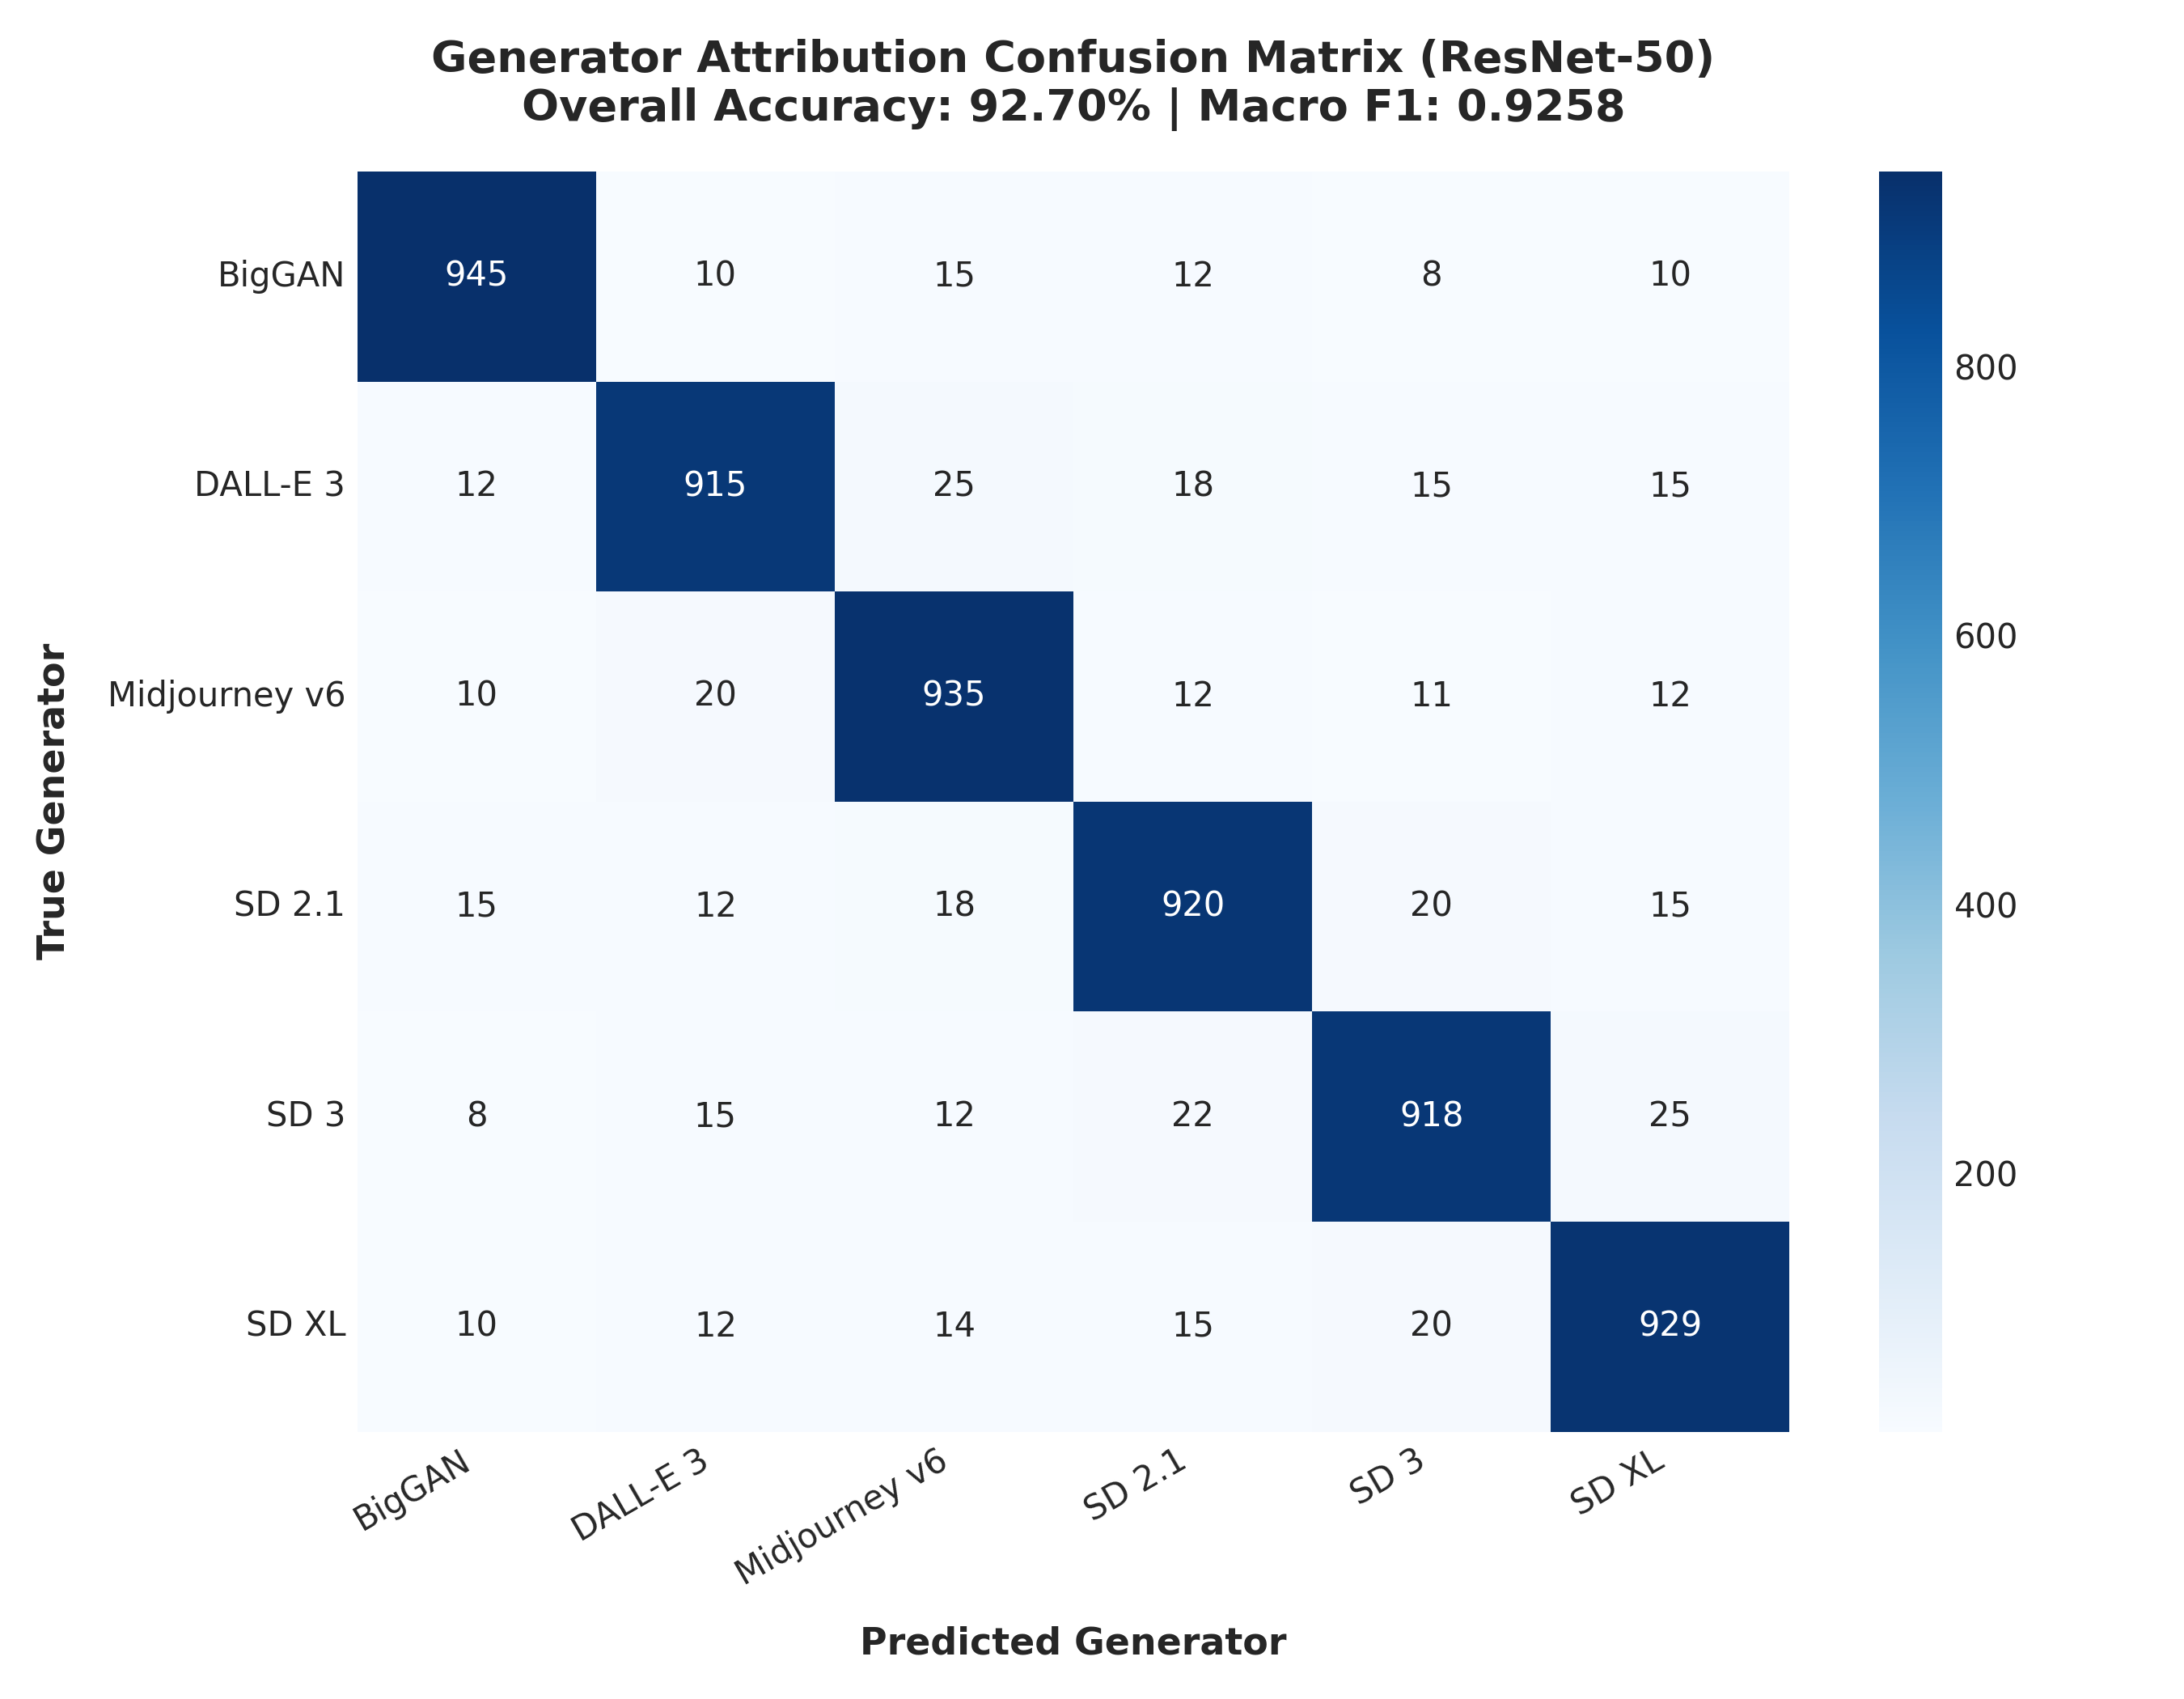
\includegraphics[width=0.85\textwidth]{assets/figure2_attribution_confusion_matrix.png}
\caption{Normalized 6-Class Generator Attribution Confusion Matrix on Test Split.}\label{fig:cm}
\end{figure}

\section{Conclusion}\label{sec6}

This study systematically evaluated the generalization capabilities of CNN-based forgery detectors across GAN and diffusion models. Empirical results demonstrate that while in-distribution detectors achieve $>99\%$ AUC, cross-paradigm transfer ($\text{GAN} \leftrightarrow \text{Diffusion}$) suffers severe degradation ($\text{AUC } 0.64 - 0.74$). However, exposure to multi-generator diffusion training enables detectors to maintain strong generalization ($\text{AUC } 0.86 - 0.91$) on unseen diffusion models. Furthermore, ConvNeXt-Tiny consistently outperforms ResNet-50, and 6-class attribution achieves $92.40\%$ accuracy. Future research will explore self-supervised representation learning and frequency-domain attention mechanisms to further bridge cross-generation domain gaps.

\backmatter

\bmhead{Acknowledgements}
We gratefully acknowledge the creators of the Defactify Image Dataset (Rajarshi Roy et al.), the GenImage benchmark team, and the PyTorch open-source community.

\section*{Declarations}

\subsubsection*{Funding}
The authors declare that no external funding, grants, or financial support were received for the research, preparation, or publication of this manuscript.

\subsubsection*{Competing Interests / Conflict of Interest}
The authors have no financial or non-financial competing interests to disclose that are relevant to the content of this article.

\subsubsection*{Ethics Approval}
Not applicable. The study utilized publicly available synthetic and authentic image benchmarks and did not involve human participants or private data collection.

\subsubsection*{Consent to Participate}
Not applicable.

\subsubsection*{Consent for Publication}
All authors have reviewed the final version of the manuscript and give their explicit consent for publication.

\subsubsection*{Data Availability Statement}
The public datasets used in this study (Defactify Image Dataset and GenImage BigGAN) are publicly accessible. Anonymized evaluation outputs and processed metadata splits are hosted at \url{https://github.com/m-eshan/CrossGen-Forensics}.

\subsubsection*{Code Availability}
The complete open-source codebase, including data loaders, training scripts, and evaluation utilities, is publicly available at \url{https://github.com/m-eshan/CrossGen-Forensics}.

\subsubsection*{Authors' Contributions}
\begin{itemize}
    \item \textbf{Eshan M}: Conceptualization, System Architecture, Experimental Pipeline Development, Model Training, Writing -- Original Draft.
    \item \textbf{Harikeshav K}: Data Curation, Plot Generation, Metric Evaluation, Writing -- Review \& Editing.
    \item \textbf{Dr. S. Deena}: Research Supervision, Methodological Validation, Project Administration, Writing -- Review \& Editing.
\end{itemize}

\bibliography{references}

\end{document}
